\documentclass[format=sigconf]{acmart}
\usepackage[utf8]{inputenc}
\usepackage{enumitem}
\usepackage{float}
\usepackage[labelfont=bf,textfont=md]{caption}
\usepackage{graphicx}
\usepackage{xcolor}
\usepackage{minted}
\usepackage{hyperref}
\usepackage[parfill]{parskip}
\usepackage[all]{hypcap}
\usemintedstyle[common-lisp]{default}
\newmintinline[code]{text}{}
\bibliographystyle{plainnat}

\hypersetup{
  colorlinks,
  linkcolor={red!50!black},
  citecolor={blue!50!black},
  urlcolor={blue!80!black}
}

\newlist{step}{enumerate}{10}
\setlist[step]{label*=\arabic*.,leftmargin=2em}

\acmConference[ELS'23]{the 15th European Lisp Symposium}{March 21--22 2023}{%
  }
\acmISBN{}
\acmDOI{}
\setcopyright{rightsretained}
\copyrightyear{2023}

\begin{document}

\title{Experience Report: Kandria - A Game in Common Lisp}

\author{Nicolas ``Shinmera'' Hafner}
\affiliation{%
  \institution{Shirakumo.org}
  \city{Zürich}
  \country{Switzerland}
}

\begin{abstract}
  In this paper we outline the experience we've gathered while developing Kandria using Common Lisp. Kandria is a video game in the ``action RPG'' genre and has been developed for Windows and Linux with the SBCL implementation. Being a video game, the project touches a unique combination of disciplines within computer science, and as such provides an in-depth and comprehensive view of the development process of a large-scale project in Lisp, and the general language ecosystem.
\end{abstract}

\begin{CCSXML}
  <ccs2012>
  <concept>
  <concept_id>10010147.10010371</concept_id>
  <concept_desc>Computing methodologies~Computer graphics</concept_desc>
  <concept_significance>300</concept_significance>
  </concept>
  <concept>
  <concept_id>10010520.10010570.10010574</concept_id>
  <concept_desc>Computer systems organization~Real-time system architecture</concept_desc>
  <concept_significance>300</concept_significance>
  </concept>
  <concept>
  <concept_id>10011007.10011006.10011066.10011070</concept_id>
  <concept_desc>Software and its engineering~Application specific development environments</concept_desc>
  <concept_significance>500</concept_significance>
  </concept>
  <concept>
  <concept_id>10011007.10011074.10011092.10011093</concept_id>
  <concept_desc>Software and its engineering~Object oriented development</concept_desc>
  <concept_significance>100</concept_significance>
  </concept>
  <concept>
  <concept_id>10011007.10011074.10011092.10011691</concept_id>
  <concept_desc>Software and its engineering~Error handling and recovery</concept_desc>
  <concept_significance>100</concept_significance>
  </concept>
  <concept>
  <concept_id>10011007.10011074.10011081.10011082</concept_id>
  <concept_desc>Software and its engineering~Software development methods</concept_desc>
  <concept_significance>100</concept_significance>
  </concept>
  </ccs2012>
\end{CCSXML}

\ccsdesc[300]{Computing methodologies~Computer graphics}
\ccsdesc[300]{Computer systems organization~Real-time system architecture}
\ccsdesc[500]{Software and its engineering~Application specific development environments}
\ccsdesc[100]{Software and its engineering~Object oriented development}
\ccsdesc[100]{Software and its engineering~Error handling and recovery}
\ccsdesc[100]{Software and its engineering~Software development methods}
\keywords{Common Lisp, Games, Video Games, Computer Graphics, Experience Report}

\maketitle

\def\abovecaptionskip{1pt}
\def\listingautorefname{Listing}
\def\figureautorefname{Figure}

\section{Introduction}\label{introduction}
Kandria is a video game in the ``action RPG'' genre that was released worldwide on the \href{https://kandria.com/steam}{Valve Steam} platform for Windows and Linux in January of 2023, receiving very positive reviews. The game was developed using the Trial engine and thus relies almost entirely upon code and libraries written in Common Lisp -- to our knowledge the first commercial game like this to be released.

\begin{figure}[h]
  \begin{centering}
    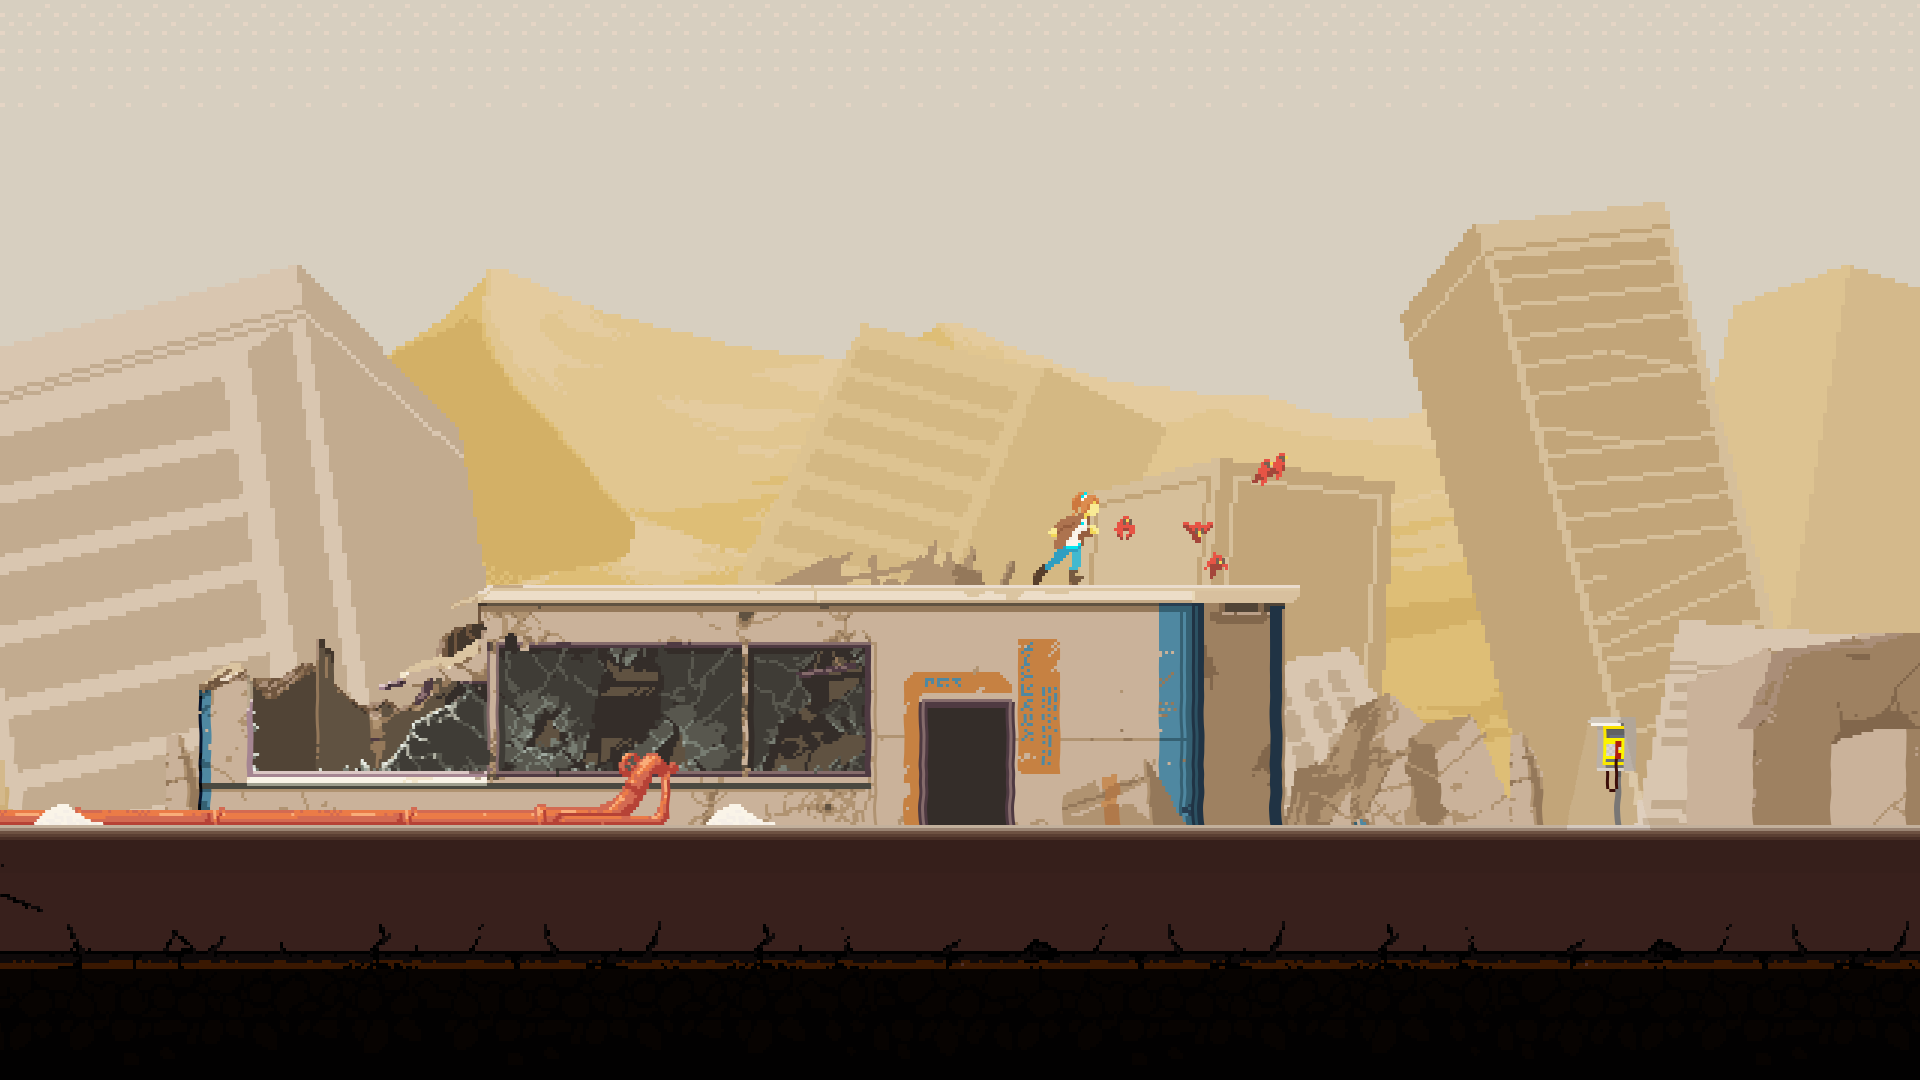
\includegraphics[width=0.4\textwidth]{screenshot 8.png}
  \end{centering}
  \caption{A screenshot of Kandria}
\end{figure}

Games lie at an intersection of many different computer science disciplines such as audio, graphics, interfaces, soft real-time, artificial intelligence, and more. As such games provide a unique challenge in combining all of these disciplines together into one product, and ultimately shipping this product to paying customers.

In this paper we will outline the challenges we faced in realising Kandria as related to Common Lisp, discuss advantages of our approach, and take a look at the work still ahead of us in expanding the capabilities of our engine to better address the requirements of even more complex games we would like to develop in the future.

In particular we will note our own experiences with a few common Boogeymen, such as the overhead of CLOS dispatch, the pause times of GC, the maturity of the library ecosystem, and the stability and size of deployed binaries.

Since this is an experience report, we cannot present any specific figures on performance characteristics, statistics on used projects, or some sort of unified thesis. Instead we hope that this insight will be valuable for readers to gain a better understanding of the complexities involved, the benefits we have identified with Lisp over other ecosystems, and, most importantly, the areas in which work still needs to be done.

All of the work we've done, including Trial, and even Kandria, is open source and available on our GitHub\cite{github}, in the hopes that it will inspire others to create new projects based upon them.

\section{Related Work}\label{relatedwork}
In \cite{hafner2021} we discussed many similar points that this paper touches upon in a format more suitable for people unfamiliar with the intricacies of lisp and especially Common Lisp.

Strandh\cite{strandh2014fast} proposes a new approach to improve the performance characteristics of generic function dispatch. Since we make heavy use of CLOS in our game, such improvements are very relevant.

Patton\cite{swcl-gc} are working on a new parallelisation of the SBCL garbage collector to allow for faster collection and thus reduced pause times. GC pause times are a frequently reported issue in games, as they can cause unexpected latency, and thus lead to drops in the framerate.

Mäkelä\cite{makela2021development} describe their experience in developing a game using the open source game engine Godot, with C\#. Godot is currently the leading open source game engine, and is striving to be a viable alternative to commercial products like Unity and Unreal.

Craighead et al.\cite{craighead2008using} cover a case study of using Unity, a proprietary game engine, to build a small game. Unity is currently most-used game engine for small to mid-sized games.

Nurminen\cite{nurminen1990rft} describe their experience developing and deploying a Common Lisp application to users.

\section{Library Ecosystem}\label{yaks}
In this section we will outline our general experience working in the Common Lisp ecosystem, and particularly the contributions we've made to it in order to implement Kandria.

Out of the 110 libraries Kandria depends upon, 54 were written by us. This does mean that we've spent a rather significant amount of time ``yak shaving'' and creating libraries to fulfil a variety of needs that were, prior to their creation, either completely unfulfilled, or unsatisfactorily so. We will go into detail on some of the more important ones in the following subsections.

While this is undeniably a lot of work, it has been done now and is available to others. Furthermore, of the other half of libraries that we were not authors of, the vast majority have been extremely stable. We only needed to supply extremely minimal patches to a select few libraries, most of which were reviewed and accepted relatively swiftly.

Among this we also count the SBCL implementation itself. While we strive to write implementation independent code in our separate libraries, for Kandria itself we decided to only focus on SBCL in order to reduce the development overhead. SBCL offers great native code performance and is available for all platform configurations that we require. And, perhaps most importantly, it is very actively maintained. Most of the issues we've encountered in releases were usually fixed within a few weeks, if not days.

We are also actively investigating the possibility of porting SBCL and Kandria to the proprietary Nintendo Switch platform, though due to Non-Disclosure Agreements we are unfortunately not at liberty to speak of the specifics involved in that at this time.

Overall while we certainly had to create a lot of libraries to fulfil our needs, and those libraries presented a significant amount of effort to implement, we remain convinced that we were only able to implement these systems in a respectable amount of time due to the convenience factors that Lisp offers us.

We'll now touch on a few specific areas that we developed libraries for. This is by no means exhaustive, but we consider these to be the most relevant to the general community.

\subsection{Math Libraries}\label{math}
While there is no shortage of math libraries available to Common Lisp, especially linear algebra implementations, most of those libraries focus on large scale scientific computing, often by integrating with foreign libraries such as BLAS and LAPACK. For basic computer graphics and especially games, this is overkill. Most of the linear algebra stays within the confines of 2x2, 3x3, 4x4 matrices, and 2, 3, and 4 element vectors.

It is more important to provide a very convenient interface that allows us to perform computations on these elements with adequate speed. Back when Trial started out, no linear algebra libraries with such a limited focus existed, and as such the 3d-Vectors and 3d-Matrices libraries were born. We have since extended this set of libraries to include 3d-Quaternions for common operations with rotations, and 3d-Transforms, for the convenient encapsulation of a ``transform gizmo'' that can represent rotation, translation, and scaling without Gimbal Lock.

All of these libraries rely very heavily on macros to reduce code duplication and automatically generate code for loop unrolling and other common tactics in linear algebra code. The current versions of these libraries all work by emitting an \code{etypecase} for every operation, which then handles dispatch based on the provided argument types. The operation functions are inlined, such that the compiler can eliminate the dispatch altogether if the argument types are locally known. This allows us to provide a generic interface to the user that's quite convenient, while still staying competitive in performance critical sections.

Unfortunately this approach, while portable, is also riddled with issues: since every operation is inlined, this leads to explosive code growth for the compiler before it can reduce the code back down again by eliminating superfluous dispatch \code{etypecase}s. Type inference is also much more complicated, and stack allocation is usually only possible via careful manual rewriting of the operations involved. The libraries are also limited to a single float type, meaning you can by default only create vectors with single-floats as elements.

In this case the lack of static typing facilities and lack of portable compiler hooks for integrating with type inference really hurts the compile speed, implementation clarity, and ultimate performance of the resulting code.

We have started work on a full rewrite of all libraries that take a fundamentally different approach: instead of emitting etypecases and relying on inlining, we create a sort of ``template mechanism'' by which we can generate all possible permutations of a singular function for all involved argument types. This gives us very tiny, but perfectly optimised base functions for all required operations. We then create a dispatcher function on top which falls back to emitting an \code{etypecase} on other implementations, but will hook into SBCL's \code{deftransform} and similar facilities to better handle expansion and type propagation. Finally we create variadic functions on top of the dispatchers which transform any possible variadic call into calls to dispatched 2-argument operation functions, while retaining proper type propagation.

Ultimately this results in much more easily understandable and performing code. However, it still comes at a cost: because we cannot know ahead of time which type combinations and operations the user will actually need, we must generate all possible combinations ahead of time. This potentially results in thousands of functions being generated that are never used. We would like a compiler facility that allows us to hook into the expansion process of a function call to generate the required permutations on-demand.

While such a facility is conceivable, and making it work for unknown runtime types by delayed compilation is, too, we currently have no plans to implement such an advanced strategy. More importantly, we hope that at some point in the future implementors can come to some kind of consensus that would allow a portability library to expose a similar mechanism to SBCL's \code{deftransform} for faster, more convenient, type-inference-informed call expansion.

\subsection{User Interfaces}\label{ui}
When Trial initially began its development in 2016 it was directly integrated with the Qt4 UI toolkit (via CommonQt / Qtools). Since Qt4 is a rather large dependency that not only increases the deployed package size, but also invites a lot of C and C++ interop that can cause hard to debug issues, and has not been maintained in many years, it was quickly abandoned, however. These days Trial does not depend on a UI toolkit directly, or even a specific backend for its OpenGL use.

Aside from CommonQt, the options for a user interface in Common Lisp were, and remain, limited: GTK runs the same issues as Qt, though with even worse deployment and support aspects, LTK is far too limited and cannot integrate with OpenGL at all, McCLIM similarly does not possess an OpenGL backend or method of integration and is still very limited in its theming capabilities, and the newly established CLOG requires a browser to be shipped, which is far too heavy-weight.

As a result we decided to implement our own toolkit, called Alloy. Alloy is separated into different protocols, with the core being completely independent of any rendering or input method, instead only handling the layouting decisions, the input handling via a generic event protocol, and a system to dynamically react to changes in the represented data.

How visual elements can be rendered is then offloaded to several other protocols: the ``Simple Rendering Protocol'' which provides a basic text and shape rendering API, the ``Presentations Protocol'' which allows users to describe how to compose the look of a visual element via the basic shapes from the Simple protocol, and the ``Animations Protocol'' which allows users to describe how shapes change over time as properties of a visual element are changed.

Finally, the Simple protocol needs to be implemented by a backend, such as the ``OpenGL Renderer'' to actually provide a way to draw the shapes in some way, the Core protocol needs to receive input events from the surrounding context to actually react to user input, and some method of rendering and layouting text needs to be provided. Text in particular is separated out as it is a very complex topic in its own right.

This separation of concerns via protocols implemented in CLOS allows us to make Alloy far more amenable to being ported to different backends. In particular, it allows us to use Alloy in contexts that are otherwise rather unusual for UI toolkits, such as within a game where the actual operating system interaction and rendering logic cannot be directly controlled by the toolkit itself, but is instead handled by the game engine.

Usual desktop UI toolkits are rather cumbersome to style effectively, as most desktop applications are expected to present themselves in a ``native look and feel'', while games are expected to have rather elaborately customised and animated interfaces. Alloy's presentations protocol allows us to style the UI quite extensively. Thanks to macros we can present the user with a declarative style interface to define these behaviours with relative ease.

This protocol separation would not be possible to implement without the high degree of flexibility CLOS offers us in combining behaviours, and even without advanced techniques such as shadow mixins and metaclasses.

\subsection{Audio Processing}\label{audio}
Of the entire system, audio processing is where the toughest constraints apply, as audio is very sensitive to latency. We cannot process audio in large buffers to smooth over processing hiccups, as then sound effects would be desynchronised from their visual counterparts. Audio processing can also often be very computation intensive, and benefits greatly from vectorisation.

For these reasons we have decided to write the main bulk of our processing as a C library, rather than Common Lisp, as at the time it was the fastest way for us to get the kinds of performance constraints met and the kinds of capabilities we needed. Now with the advent of the sb-simd contrib, writing a competitive alternative (albeit constrained to SBCL) may be feasible.

In any case, our library, libmixed, follows a very strict C style and is extensible and interoperable from Lisp. You can write ``segments'' that process audio from Lisp as well, and integrate with the rest of the processing system neatly.

This allows us to write the more hairy parts such as audio format decoding, and audio playback in Lisp, instead, without sacrificing the performance gains in the bulk of the processing. Libmixed then takes care of unpacking and decoding audio streams, applying a variety of effects, mixing multiple audio streams together, and even resampling everything to fit into the expected, and often differing, sample rates at the input and output points.

Libmixed also includes a full introspection API, allowing us to not only put the audio processing pipeline together from Lisp, but also to interactively inspect the state of the processing segments and modify them at runtime. We can also use the extensibility to prototype new effects from Lisp before lowering them down to C should the performance requirements be strict enough.

On the Lisp side we have also crafted a more high-level system called Harmony, which makes it trivial to put together these processing pipelines, and interactively play music and sound effects back. In Kandria we use these pipelines for a variety of effects such as cross fading multiple music layers (called ``horizontal mixing''), ducking the audio with a low pass filter when the player is under water, and slowing down audio playback when the player enters a slow motion segment.

\subsection{Operating System Interaction}\label{os}
In order to output sound and graphics, process input, and receive user information we need to interact with the surrounding operating system. On all three targets we care about, this is done via calls to a C API of some sort. Thanks to CFFI it is usually unnecessary to actually rely on an external C library to do so, and we can instead code the interaction directly in Lisp, retaining the interactive implementation and debugging.

Despite this though, the interaction still involves C and the usual memory safety perils, and depending on the interface the documentation often leaves things to be desired, especially on MacOS. So while our implementation definitely benefits from a much faster retry cycle, it is still a very arduous process to write these OS interop libraries.

Particularly we had to write libraries to do the following:
\begin{enumerate}
\item Input handling for game controllers. This is rather involved, especially on Windows, where multiple APIs need to be supported simultaneously.
\item Audio output. We've implemented several different output APIs on both Linux and Windows, as both systems can differ on their supported output interfaces depending on version and setup.
\item Native dialog boxes. In order to show emergency error boxes or prompt the user for files.
\item Font discovery. To search the available fonts for a matching set we need to query operating system APIs.
\item Language querying. To ensure the game launches with the user's language (if supported of course), we again need to query the environment for the preferred localisation.
\end{enumerate}

For graphics output and general window interaction we currently rely on the GLFW C library, as it has proven extremely stable and portable. It is conceivable that we will replace this at some point to reduce C dependencies, but given that we've had zero issues arising from its use, this is rather low priority for us.

\subsection{Service Integration}\label{steam}
In order to publish a game on the Steam platform, you must integrate with their SteamWorks SDK. The actually required amount of integration is very minimal, and merely involves loading their shared library and calling a single function. However, the SteamWorks SDK offers a lot of other functionality that games can make use of, like social networking features, user generated content sharing, multiplayer systems, and more.

Unlike the prior OS interfaces, the default expected interaction mode with the SteamWorks SDK is via C++, which is quite difficult to talk with directly via CFFI. Fortunately, they also offer a raw C API, but this API is not fully documented and fraught with strange gotchas. The SDK does ship a ``machine readable'' description of the endpoints, structures, and types in the form of a JSON file, but as we have found this file is both incomplete and partially incorrect.

In our implementation we analyse the JSON file along with a manually supplied file with the lacking data, and a couple of the shipped static headers to automatically generate the CFFI wrapper data structures, types, constants, and functions. Since the analysis of these files is rather involved however, we have chosen not to use macroexpansion, but rather provide a separate system which emits Lisp code to a new file.

In addition to this generated interface, we also had to supply a minimal ``shim'' C library that handles a few select API calls that rely on structure-by-value passing, a feature which is not natively supported on most Lisp implementations at this point. Another workaround would be to use libffi, but libffi comes with its own issue, and would be another C library to depend on anyhow, so we opted for the much simpler and easier to understand alternative of writing our own minimal shim library.

In Kandria we make use of the extended services to present the user with an on-screen keyboard when they are using a controller, to read out the username for default save file naming, and to integrate with the Steam platform's ``achievements'' system, which players have come to expect.

\section{Common Lisp Object System}\label{clos}
In both Trial and Kandria we make rather extensive use of CLOS, both its basic features of classes, multiple dispatch, and deep hierarchies via mixins, and the advanced features of metaclasses. For instance, our entire event handling system is simply a singular function \code{(handle event receiver)} which we define methods on to receive events. A central ``event loop'' object then just calls the handle function for every event it receives on every receiver it has in its internal list.

As described in our prior paper \cite{hafner2018} we use metaclasses to attach ``shader fragments'' (code that is executed on the GPU during rendering) to classes and inherit the behaviour of these fragments together, allowing composition of rendering behaviour through inheritance as well.

Overall the use of classes as an organisational structure lends itself extremely well to games, especially in the presence of multiple inheritance and mixins. We also often use this to introduce ``marker classes'' that contain no behaviour or data of their own, but act as type information that other parts of the system use, such as whether a class can be instantiated by the editor, resized, should be treated as solid during collision, should not be deleted when loading a prior save state, etc.

We make use of structures over standard objects only in very select cases where the impact of the increased verbosity can be contained, and the performance requirements actually indicated that we needed to optimise. Specifically this is for the hit information during collision resolution, for the node graph that powers the pathing AI, and the glyph information used for text layouting and rendering. In those cases the initial class approach produced too much overhead with repeated slot access dispatch, so we switched to a few specific structures.

Especially with regards to propagating type information CLOS can be a hindrance, as you are prevented from declaring the argument and return types. Structures give us the advantage of fixing a return type on their accessors, propagating type information more easily and thus leading to better performing code at their call sites. There are projects that allow inlining method dispatch as well, eliminating some of the type ambiguity, but we have not seriously investigated these approaches yet.

Overall the dispatch overhead of CLOS has never been a real problem for us. Even with thousands of objects that receive events through our \code{handle} function, hundreds of methods attached to it, and tens of events every frame, not to mention all the other parts in the game that use CLOS, we still manage to easily hit a steady 120 frames per second on a ten year old machine.

\section{Performance \& Garbage Collection}\label{performance}
Overall we have needed to do surprisingly little actual performance analysis and optimisation work to make Kandria run well. This is definitely in large part thanks to SBCL's quite good native code compiler and type inference systems, and the prior work we've done to design critical libraries to not be completely obscene in terms of their performance characteristics.

We have done larger scale rewrites of several subsystems in Trial, which have provided us with general performance increases, though these rewrites were primarily done to increase the code clarity and usability, with the performance being a nice bonus.

As usual, far more important than constant factor improvements like those has been reducing the asymptotic behaviour. Introducing a Bounding Volume Hierarchy to speed up spatial queries and especially collision detection from a primitive quadratic search down to a logarithmic one has definitely provided the most significant performance improvement.

While asymptotic behaviour improvements will be applicable for projects in any language, with SBCL we've had the definite advantage of being able to rely on the statistical profiler to determine hot spots in the code. This is especially advantageous in Lisp as we can turn the profiler on and off at any time, to capture exact segments that we are interested in, rather than having to capture the full run of a program and then massaging the data manually.

Newly developed tools to better visualise the data gathered by the statistical profiler, such as the ``flamegraph'' visualiser developed by Jan Moringe have also been invaluable in gaining a better understanding of the performance characteristics of the code.

As outlined in \autoref{math} above, there are still areas in which Lisp struggles to be truly competitive, largely in part due to its very dynamic typing, an aspect that is otherwise very advantageous for development. We've also encountered issues in eliminating superfluous consing, as many convenient styles of writing code will prevent stack allocation and other garbage elimination.

We have managed to keep our garbage production down largely with two tricks:

\begin{itemize}
\item Pooling and preallocation. By storing objects in a pool and manually allocating and freeing them we can avoid allocating them at runtime, leaving less work for the GC to deal with. Since the objects are long lived, they will also be quickly promoted to later generations, lessening the work to scan other generations. The obvious downside is that we lose automatic freeing and may introduce double-use cases, but for many cases the lifetimes of the objects can be predetermined and managed relatively painlessly.
\item Using \code{load-time-value} in lieu of stack allocation. With this trick we can allocate a ``local object'' that will be modified at runtime rather than allocated fresh. The downside of this approach is that whichever function provides the load-time-value object cannot be called concurrently, and the programmer must be vigilant in tracking the lifetime of the load-time-value object should it escape the dynamic extent of the function.
\end{itemize}

We are also very interested in a recent proposal to add memory arenas to SBCL, which would allow us to capture all of the objects allocated within a dynamic extent and free them immediately on exit, further lessening the burden of the global GC in cases where we know the exact lifetimes.

Aside from memory arenas, we're also very interested in recent work by Hayley Patton to parallelise SBCL's garbage collector, though it is currently unknown when this feature will become mature and be merged into mainline SBCL.

In general we have not felt that we've had to do a lot of work to keep garbage production down. On a usual system the GC seems to trigger every ten second or so, with no noticeable stutters caused by the pause time. We have been made aware of some rare systems on which the GC pause \textit{does} cause visible stutters, but have not been able to identify why that should happen or what to do about it. Completely eliminating all runtime garbage production does not seem like an effective way to spend our time, however.

\section{Deployment}\label{deployment}
Finally we would like to talk about our experience actually delivering Kandria to users and the process we have developed for doing so.

The first step in the deployment pipeline is the build of the actual game binary, for which we use the ASDF build system and the Deploy library. With these all game code is compiled fresh, dumped into an executable suitable for the local platform, and bundled together with the depended-upon shared libraries, producing an executable ready for deployment to target machines.

However, since the build does not happen from scratch via a platform independent compiler, we have to ensure that we use an SBCL version that has been compiled on our minimal target platform version. For instance, we build the SBCL we use for deployment in a virtual machine on an old Linux version to ensure that internal symbol version dependencies in glibc can be satisfied on target machines. We have to take similar care for all required shared libraries that are shipped. Once this version has been compiled however, we can simply invoke it on any Linux version we like to use, and don't have to build the entire system inside a VM.

We can also directly build Windows version of the game on Linux by using WINE. This has worked flawlessly for us, and we imagine that it would also be possible to do the inverse on Windows by using the Windows Subsystem for Linux to build Linux versions of the games. We've also investigated the possibility of using Darling to build MacOS versions. Unfortunately Darling is not able to run SBCL as of the writing of this paper.

For all generated binaries we also make use of SBCL's core compression to reduce the binary size to about 35MB per platform. The newly introduced support for zstd also brings improved compression rates and startup speeds over the older zlib. This binary size is more than acceptable to us and is completely dwarfed by the resource files for sound and graphics.

We also make use of hooks in the Deploy library to extract these resource files from their source directory and bundle them alongside the binary when building. Paths to resource files are resolved at runtime in the engine, and are thus trivial to redirect to binary-relative paths when deployed.

Finally we have created a release system that invokes the necessary SBCL subprocesses to kick off a build, prunes out unnecessary files from the generated release, then bundles it all into a ZIP for easy delivery to testers. The system can also upload the release directly to a variety of distribution platforms including Steam, Itch.io, Keygen, and generic HTTP or FTP servers. Ultimately this allows us to compile, bundle, package, and upload new builds with a single command, drastically reducing the time and complexity involved in supplying testers and users with bugfixes.

Another aspect that is advantageous to Lisp's dynamic nature is that when an unhandled condition occurs on a target system we can, in almost all cases, still use the system well enough to gather telemetry and submit an automated crash report. This has been invaluable for us to detect rare bugs, especially ones related to uncommon system configurations that we would otherwise never have been able to catch.

\section{Conclusion}\label{conclusion}
Overall the biggest hurdle we have had in our development of Kandria has nothing to do with the language itself, but rather with the general lack of manpower behind the community. We have had to spend large amounts of time implementing, testing, and documenting auxiliary systems that have often close to nothing to do with the core process of implementing a game. This is also why we have been extremely light on topics that concern the actual game implementation process in this paper.

On the other hand, it is very clear to us that interactive development is an immense boon to the development of a game. Being able to redefine game behaviour at runtime to quickly iterate on the game content and feel is invaluable. So much so that almost every engine in use will have some form of scripting language available for game logic specifically, such that designers can iterate quickly. However, having the full stack of code available, debuggable, and performing just as well as any other part of the system is undeniably far more convenient.

We also fully recognise that while Kandria is a full game project, it is by its nature rather limited in the required processing capabilities. A lot more work is needed to support more complex games, which we intend on focusing on in the near future. However, we do not at present see any deal breakers that would make it unfeasible to create such games using Common Lisp and the base ecosystem we have helped establish so far.

If anything the recent advances in SBCL's capabilities show us a very promising future and we are excited to make use of them to further improve the situation, and with much of the ``grunt work'' now done we should be able to focus our efforts onto problems more directly associated with game development instead.

\section{Further Work}\label{further-work}
Currently a sizable amount of work in Kandria has not been backported into Trial for more general purpose use. We would like to extract a few of the systems and generalise them to make them available for other users.

We are also working on implementing several new subsystems in Trial to allow creating 3D games, as well. A skeletal animation system has been completed, and we're currently working on a physics subsystem. Also needed will be several spatial query structures to speed up collision testing, along with a more unified rendering subsystem to support Physics Based Rendering pipelines.

Finally we are also exploring the possibility of porting the engine to work on closed platforms such as the Nintendo Switch. This presents several challenges that we unfortunately cannot elaborate on here due to non-disclosure agreements.

\section{Acknowledgements}\label{acknowledgements}
We would like to thank \textit{you} for being beautiful and nice :)

Kandria was funded in part by the Pro Helvetia Interactive Media Grant and the KPT Poland Prize Digital Dragons Accelerator.
\bibliography{paper}
\end{document}

%%% Local Variables:
%%% mode: latex
%%% TeX-command-extra-options: "-shell-escape"
%%% TeX-master: t
%%% TeX-engine: luatex
%%% End:
